\chapter{Comparative estimation} 

\label{Chapter 2}
\lhead{Chapter 2. \emph{Estimation}}
\vspace{3cm}
\newpage

% New Sections for Ami to read
% - Introduction
% - Discussion

\noindent
The method, results and discussion of this Chapter appear as Appendix A of the published manuscript `comparative estimation systems perform under severely limited capacity' \cite{garrett2019comparative}. I would like to acknowledge the work of Laura A. Waters and Alexander Thorpe, in assisting with data collection for this thesis chapter. 

\color{\Red}
\section{Chapter aims}
In this Chapter, we aimed to develop a new experimental design that merges a comparative estimation task with the double-factorial paradigm --- a requirement of SFT. The double-factorial paradigm, as designed by Townsend \citeyear{Townsend_1995}, requires two levels of manipulation: load and salience. The manipulation of load is manifested by factorial manipulation of signal x presence, such that there are typically four resulting conditions: target-signal A present, B present, both present, or none. A second manipulation of salience --- nested within the manipulation of load --- must selectively influence the discriminability of the target, making high-salience targets easier and faster to respond to than low-salience targets. In addition to these `standard' requirements of the double-factorial paradigm, our novel design must engage the approximate number system in order to answer fundamental questions regarding systems of comparative estimation (as applied in Chapter 3). We begin with a brief introduction on how estimation tasks and the approximate number system are typically measured, before showcasing a novel experimental procedure designed to address the aims of this chapter.

\section{Assessments of estimation}
Estimation acuity is typically assessed through the self-report method. Participants are presented a range of item-set sizes and using a number-pad, report their estimates of quantity. The self-report method has three advantages: the task is simple, reliable, and may help establish if the approximate number system is being engaged \cite{Whalen1999, Cordes2001}.

Establishing ANS engagement is critical to any future assessment of comparative estimation systems. When we compare two quantities, we may i) estimate the quantity of each item-set, or ii) compare low-level perceptual covariates of quantity, such as area or density, to inform our decisions \cite{dehaene2011NumSense}. Since density and area are covariates of quantity, this strategy may lead to an accurate response while not engaging the ANS. For the purposes of assessing systems of comparative estimation, we must ensure estimates are performed using the ANS and not low-level perceptual covariates of quantity. 

One method of measuring ANS engagement is through the self-reported coefficient of variance. As previously noted, the ANS follows a logarithmic scale. When the ANS is engaged in a self-reported estimation-task, the mean and standard-deviation of response-estimates increase in a linear fashion with the number of items to be enumerated. This results in a coefficient of variance (standard-deviation divided by the mean) ranging from approximately 0.14 to 0.4 \cite<see>{Whalen1999, Cordes2001, HALBERDA_2006}. This method provides a measure of ANS engagement, but at a cost to the fidelity of estimation response-time.

% AE: perhaps say in a sentence above how the coefficient of variance is calculated ?
% PG: Done

When a participant self-reports a numerical estimate, it is unclear at what time the cognitive processes behind their decision terminated. For example, does a decision terminate when a participant finishes typing their estimate? Or does a decision terminate when the participant begins typing their estimate? Might a participant change their decision as they are typing, and how does this factor into the response-time? While self-reported estimates are useful for assessing ANS engagement, this method provides a poor assessment of ANS decision time. This is a problem for the primary tools of SFT --- the SIC and capacity coefficient --- that rely on response-time distributions. The self-reported method has a further limitation, in that it cannot conform to the binary `yes' and `no', target-present vs target-absent response-set necessary for SFT. To address these limitations, we consider an alternative numerical task.

\subsection{The comparative numerosity task}
An alternative method for assessing response-times using a binary response-set while potentially engaging the ANS, is a comparative numerosity task \cite{leibovich2014comparing,pansky2002comparative,piazza2004}. Here, subjects are asked whether an item-set is greater-than or less-than a specified criterion, to which a binary `yes' or `no' response is provided. In this response-format, decision-time and response-time are tied to a single key-press, creating a more reliable measure of decision finishing-time. Furthermore, the comparative numerosity task is designed to engage and measure a specific aspect of the number system: the numerical distance effect \cite{buckley1974comparisons}. 

Under the numerical distance effect, item-sets that are closer together are harder to relatively estimate than item-sets that are further apart \emph{i.e}., estimating whether 22 items are greater-than 20 items is harder than estimating whether 30 items are greater-than 20 items \cite{moyer1967time}. As such, closer item-sets incur a reliable penalty to response-time and accuracy. This makes the numerical distance effect a useful manipulation of difficulty (salience), in a task that requires a stable manipulation of response-time, such as SFT. The next challenge is in merging this comparative numerosity task with the necessary double-factorial paradigm used in SFT. 

\subsection{The double-factorial numerosity task}
The comparative numerosity task can be modified to meet the requirements of the double-factorial paradigm (see Figure \ref{fig:EgIllus}.a as an example). Target item-sets can be defined as being less-than a specified criterion, creating a binary `target-present' vs `target-absent' manipulation of load (for example, Figure \ref{fig:EgIllus}.b)\footnote{Typically, a greater-than criterion is used in comparative numerosity task \cite{piazza2004,price2012,libertus2016, leibovich2014comparing,pansky2002comparative} as it aligns with the size- and semantic-congruency effects; however, as the reader will soon find, a less-than criterion works equally well and becomes necessary in Chapter 4 when comparing smaller quantities, (i.e., subitizing).}. A double-target trial would be two item-sets, both less-than the criterion. Each `channel' or item-set, could be identified by set-color, for example, red or blue discs (see Figure \ref{fig:EgIllus}.c). Target salience can be manipulated by the numerical distance effect with target quantities close to the criterion incurring a reliable cost to response-time, relative to quantities that are further away. This task design meets the requirements of the double-factorial paradigm, yet, introduces a new complication: the target-absent channel.

\begin{figure}[hbt]
\centering 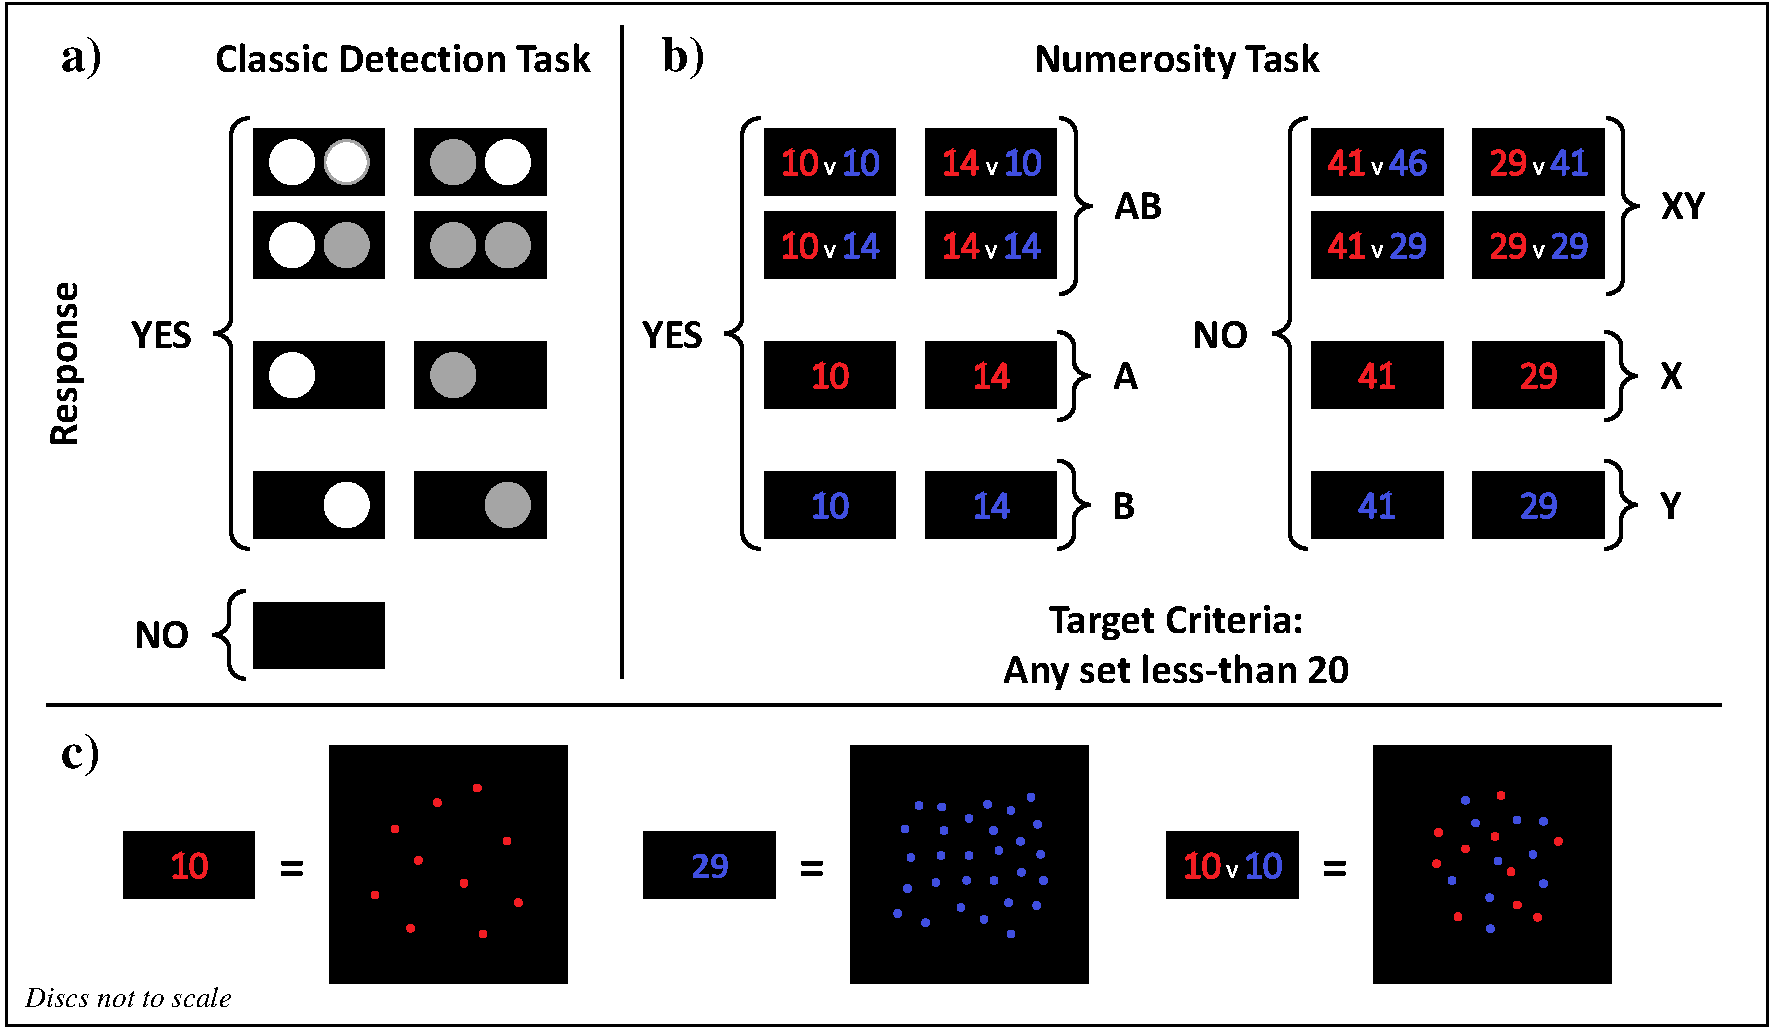
\includegraphics[width=\linewidth]{Figures/Estimation/ExampleIllustration.pdf}
\caption{Illustration of a) stimuli and correct responses for the classic `OR' detection task (Townsend \& Nozawa, 1995), b) colored digits symbolizing example quantities for the proposed double-factorial numerosity task, c) illustrative example of what these symbolic values would look like. A, B and AB refer to single-target and double-target trials; X, Y and XY refer to single-distractor (target-absent) and double-distractor trials.}
\label{fig:EgIllus}
\end{figure}


% AE: i think the above section needs a CONCRETE illustration and can be aided by an exmaple figure of th estimuli used
% PG: Done.

The classical \citeA{Townsend_1995} double-factorial design (Figure \ref{fig:EgIllus}.a) was created as a detection task, however, this design is not applicable to estimation. In our task, participants must encode the quantity of a stimulus and not terminate their response via stimulus detection. \citeauthor{eidels2010stroop} encountered a similar issue enforcing the semantic processing of word stimuli. To encourage stimulus encoding, \citeauthor{eidels2010stroop} introduced distractor stimuli.

In the context of a less-than comparative numerosity task, a distractor stimuli would be any quantity greater than the criterion. For example, given a criterion of 20, a quantity of 14 would be a target and a quantity of 29 would be a distractor (see Figure \ref{fig:EgIllus}.b, right). Note, the term `distractor' here is specific to the SFT literature; the stimulus need not distract the participant, but rather enforce full encoding of the target item. Following the methodology of \citeauthor[(but see also, Little, Eidels, Fifić \& Wang, 2018\nocite{Little2018_CCF})]{eidels2010stroop}, the salience of the distractor quantities may be manipulated in a similar fashion to the target quantities. This would produce high- and low-salience target and distractor stimulus sets.

The distributional response-time tools of SFT --- the SIC and capacity coefficient --- rely on a large number of high-accuracy trials, with a significant response-time difference between high- and low-salience conditions. As such, target and distractor salience levels must meet two criteria within the double-factorial design. There must be a significant effect of response-time between high- and low-salience conditions and response accuracy should be high (\ie $\geq$90\%) at both levels of salience. 

\section{The current study}
So far in this Chapter, we have described how a comparative estimation task, implemented in a double-factorial design must i) engage the ANS, ii) use a comparative numerosity task, iii) use both target and distractor quantities, and iv) produce a significant response-time effect between the levels of salience while maintaining high response accuracy. The remainder of this Chapter will be dedicated to two experiments, specifically designed to address these requirements. 

In the current study, participants viewed a single item-set entirely composed of either red or blue discs. Participants completed two separate tasks -- a self-reported estimation task and criterion judgement task (a precursor to the comparative estimation task). In the self-report task, participants freely reported their estimates of quantity with a number pad. In the criterion judgement task, participants judged whether a presented item-set was less-than a criterion of 20 items. ANS engagement was established using the coefficient of variance as measured by the self-reported estimation task. The numerical distance effect --- our measure of salience --- and response accuracy were assessed relative to the criterion in the criterion judgement task. ANS engagement was inferred for the criterion judgement task by comparing results to the self-report task. In both tasks, quantities ranged from 10--46. This meant items were presented both above and below the central criterion of 20 items in the criterion judgement task. Together, these tasks ensured ANS engagement, assessed how numerical distance affected response-times and accuracy within the range of estimation, and provided an informed selection of high- and low-salience stimuli for the double-factorial design applied in Chapter 3.

\color{black}

\section{Method}
\subsection{Participants}
Participants were 20 undergraduate students ($F$ = 16) from the University of Newcastle. Participants were reimbursed two course credits over a one hour testing session. Participants reported as not being color blind, and as having normal or corrected-to-normal vision. The mean age was 24.4 years ($SD$ = 9.09).

\subsection{Stimuli and apparatus}
Testing was conducted in the Newcastle Cognition Laboratory. Stimuli were presented on a 21.5inch Dell S2240L (60Hz) monitor. Stimuli were generated on a Dell Optiplex 7040 computer using python 2.7.14 and the Pygame 1.9.2b package. Responses were made using a standard `qwerty' keyboard.

Stimuli comprise a single set of uniformly sized, non-overlapping discs. The item-set (disc) color was either entirely red or blue. Each disc was located randomly within a central circular field of view. At a viewing distance of 60 cm, each disc subtended a visual angle of 0.14 degrees (0.15 cm), while the circular field of view subtended a visual angle of 9.52 degrees (10 cm). Stimuli were presented on a black background. Red and blue color sets were matched for value and chroma using the Munsell color scheme \cite{Cochrane2014}, and varied only by hue. Contrast and brightness effects were further controlled using a GLoptic spectis 1.0 photometer. Red and blue colors had RGB values of [241, 29, 34] and [64, 79, 223] respectively. 

Stimulus set-sizes were logarithmically spaced to reflect the approximate number system. Item sets contained either 10, 11, 12, 13, 14, 16, 18, 22, 24, 27, 30, 33, 37, 41 or 46 discs. In the criterion judgement task, target item-sets comprised less-than 20 items and non-target item-sets comprised greater-than 20 items. This resulted in seven target and eight non-target item-sets within this task type, all within the range of estimation. 

\subsection{Procedure}
Each participant completed two within-subject response tasks, a self-reported estimation task and a criterion judgment task, over one 60 min experimental session. During the self-report task, participants used the number pad to report their estimate for the total number of discs presented on a given trial, before pressing the enter key to end the trial. During the criterion judgment task participants reported the presence of a target item-set --- those containing fewer than 20 discs --- with the `z' key, and the presence of non-target item-sets --- those containing more than 20 discs --- with the `/' key. Task order and response-keys were counter balanced between participants.

Participants completed a practice block and five experimental blocks for each task. Each block contained 60 trials, with the probability of presenting each item-set equated within a block. Accuracy feedback, `correct' or `incorrect', was displayed at the end of each practice trial within the criterion task. The true item-set numerosity was displayed at the end of each practice trial during the self-report task. Feedback was not provided during experimental blocks. Each participant completed 300 self-report experimental trials and 300 criterion judgment experimental trials. 

The progression of a trial was the same regardless of the experimental task. On a trial, participants viewed a central fixation cross for 500 ms (0.28 x 0.28 degrees visual angle) followed by a 500 ms blank. Then, participants viewed a stimulus item-set for 1000 ms followed by a backwards mask for 500 ms. Participants had 10,000 ms to respond from the onset of the stimulus. The blank screen inter stimulus interval (ISI) was 500 ms.

\subsection{Data Analysis}
Differences between conditions of set-size were assessed at the group level. Participants were excluded if accuracy in the comparative judgment task was less than 90\% in either the highest (46) or lowest (10) set-size conditions. In the self-report task, trials were excluded from analysis if the time-difference between the first numeric key-press and the enter-key exceeded 2 standard-deviations of the mean. This method removed excessively long responses where subjects may have changed their decision after starting their response. During the criterion-response task, trials that exceeded $\pm$2SD of the mean response-time were excluded. Mean RT differences between set-sizes in the comparative judgment task were assessed using paired sample \textit{t}-tests, calculated in Matlab 2015b.

\section{Results}
\subsection{Self-report task}
One participant was excluded from the analysis of both tasks due to accuracy being less-than 90\% in the largest set-size condition of the comparative judgment task. The mean and standard-deviation of self-reported response-estimates are presented in Figure \ref{fig:Ch2_ANScoefVar}. In line with expectations from the approximate number system, subjects displayed a log-linear increase in both the mean and standard-deviation of response-estimates with a coefficient of variance equal to 0.18. This coefficient of variance falls within the range predicted when the ANS is engaged.

\begin{figure}[htb]
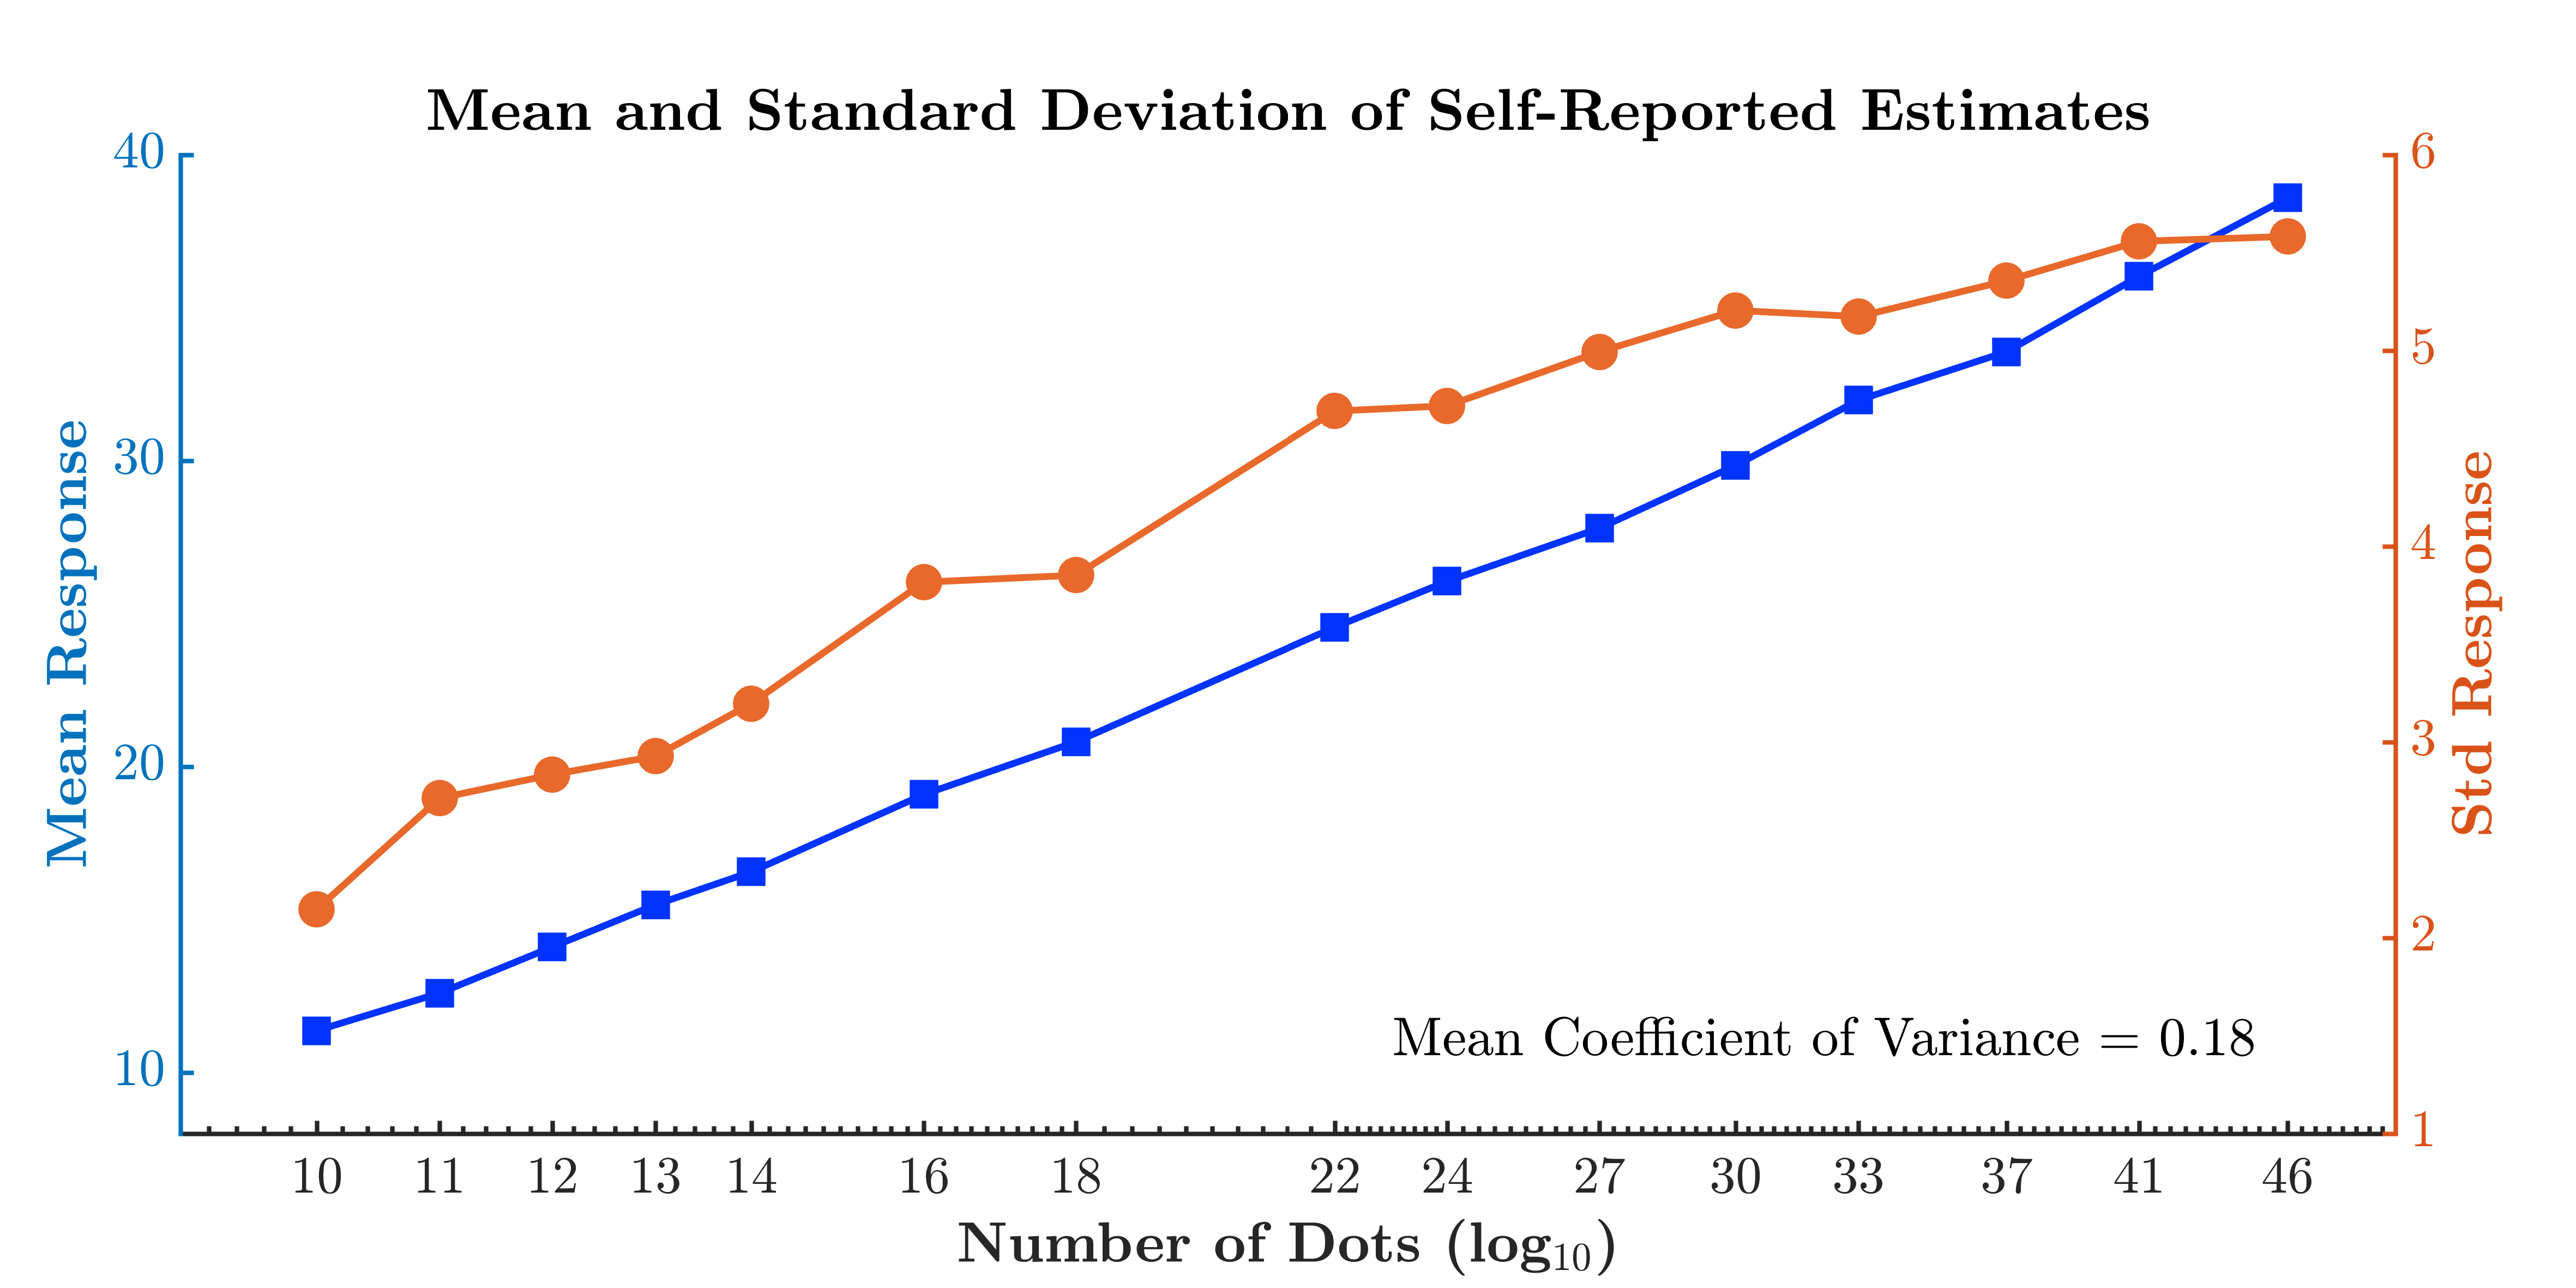
\includegraphics[scale=.4]{Figures/Estimation/CoefVar.png}
\caption{Mean (blue) and standard-deviation (orange) of self-reported response-estimates across set sizes 10--46 plotted on a log$_{10}$ scale. The mean and standard-deviation of response-estimates increase in a log-linear fashion with set-size. The mean coefficient of variance was equal to 0.18 and ranged between 0.15--0.22. This log-linear increase in the mean and standard-deviation of estimates, and a coefficient of variance falling between 0.14 and 0.4, aligns with predictions of the approximate number system.}
\label{fig:Ch2_ANScoefVar}
\end{figure}

% AE: would it be worth to plot in this figure a dotted line that marks perfect calibration (ie, where response = stimulus) to let the reader see the calibration, or lack of ?
% The Figure becomes a bit messy when I do this and it's not critical to the interpretation.

\subsection{Comparative judgment task}
At the group level, accuracy was highest at set-sizes 10 ($M$ = .98, $SD$ = .09) and 46 ($M$ = .99, $SD$ = .06), and decreased to the lowest accuracy at set-size 22 ($M$ = .59, $SD$ = .38; see top panel in Figure \ref{fig:CritVsExact}). Likewise, mean RT was fastest at set-sizes 10 ($M$ = 520 ms, $SD$ = 80 ms) and 46 ($M$ = 514 ms, $SD$ = 78 ms), and peaked at set-size 22 ($M$ = 760 ms, $SD$ = 180 ms; see middle panel in Figure \ref{fig:CritVsExact}). Both accuracy and response-time trends support the presence of a numerical distance effect, with estimation becoming less accurate and slower for item-sets closer to the criteria of 20. No speed-accuracy trade off was observed between item-sets. 

\begin{figure}[hbt]
\centering 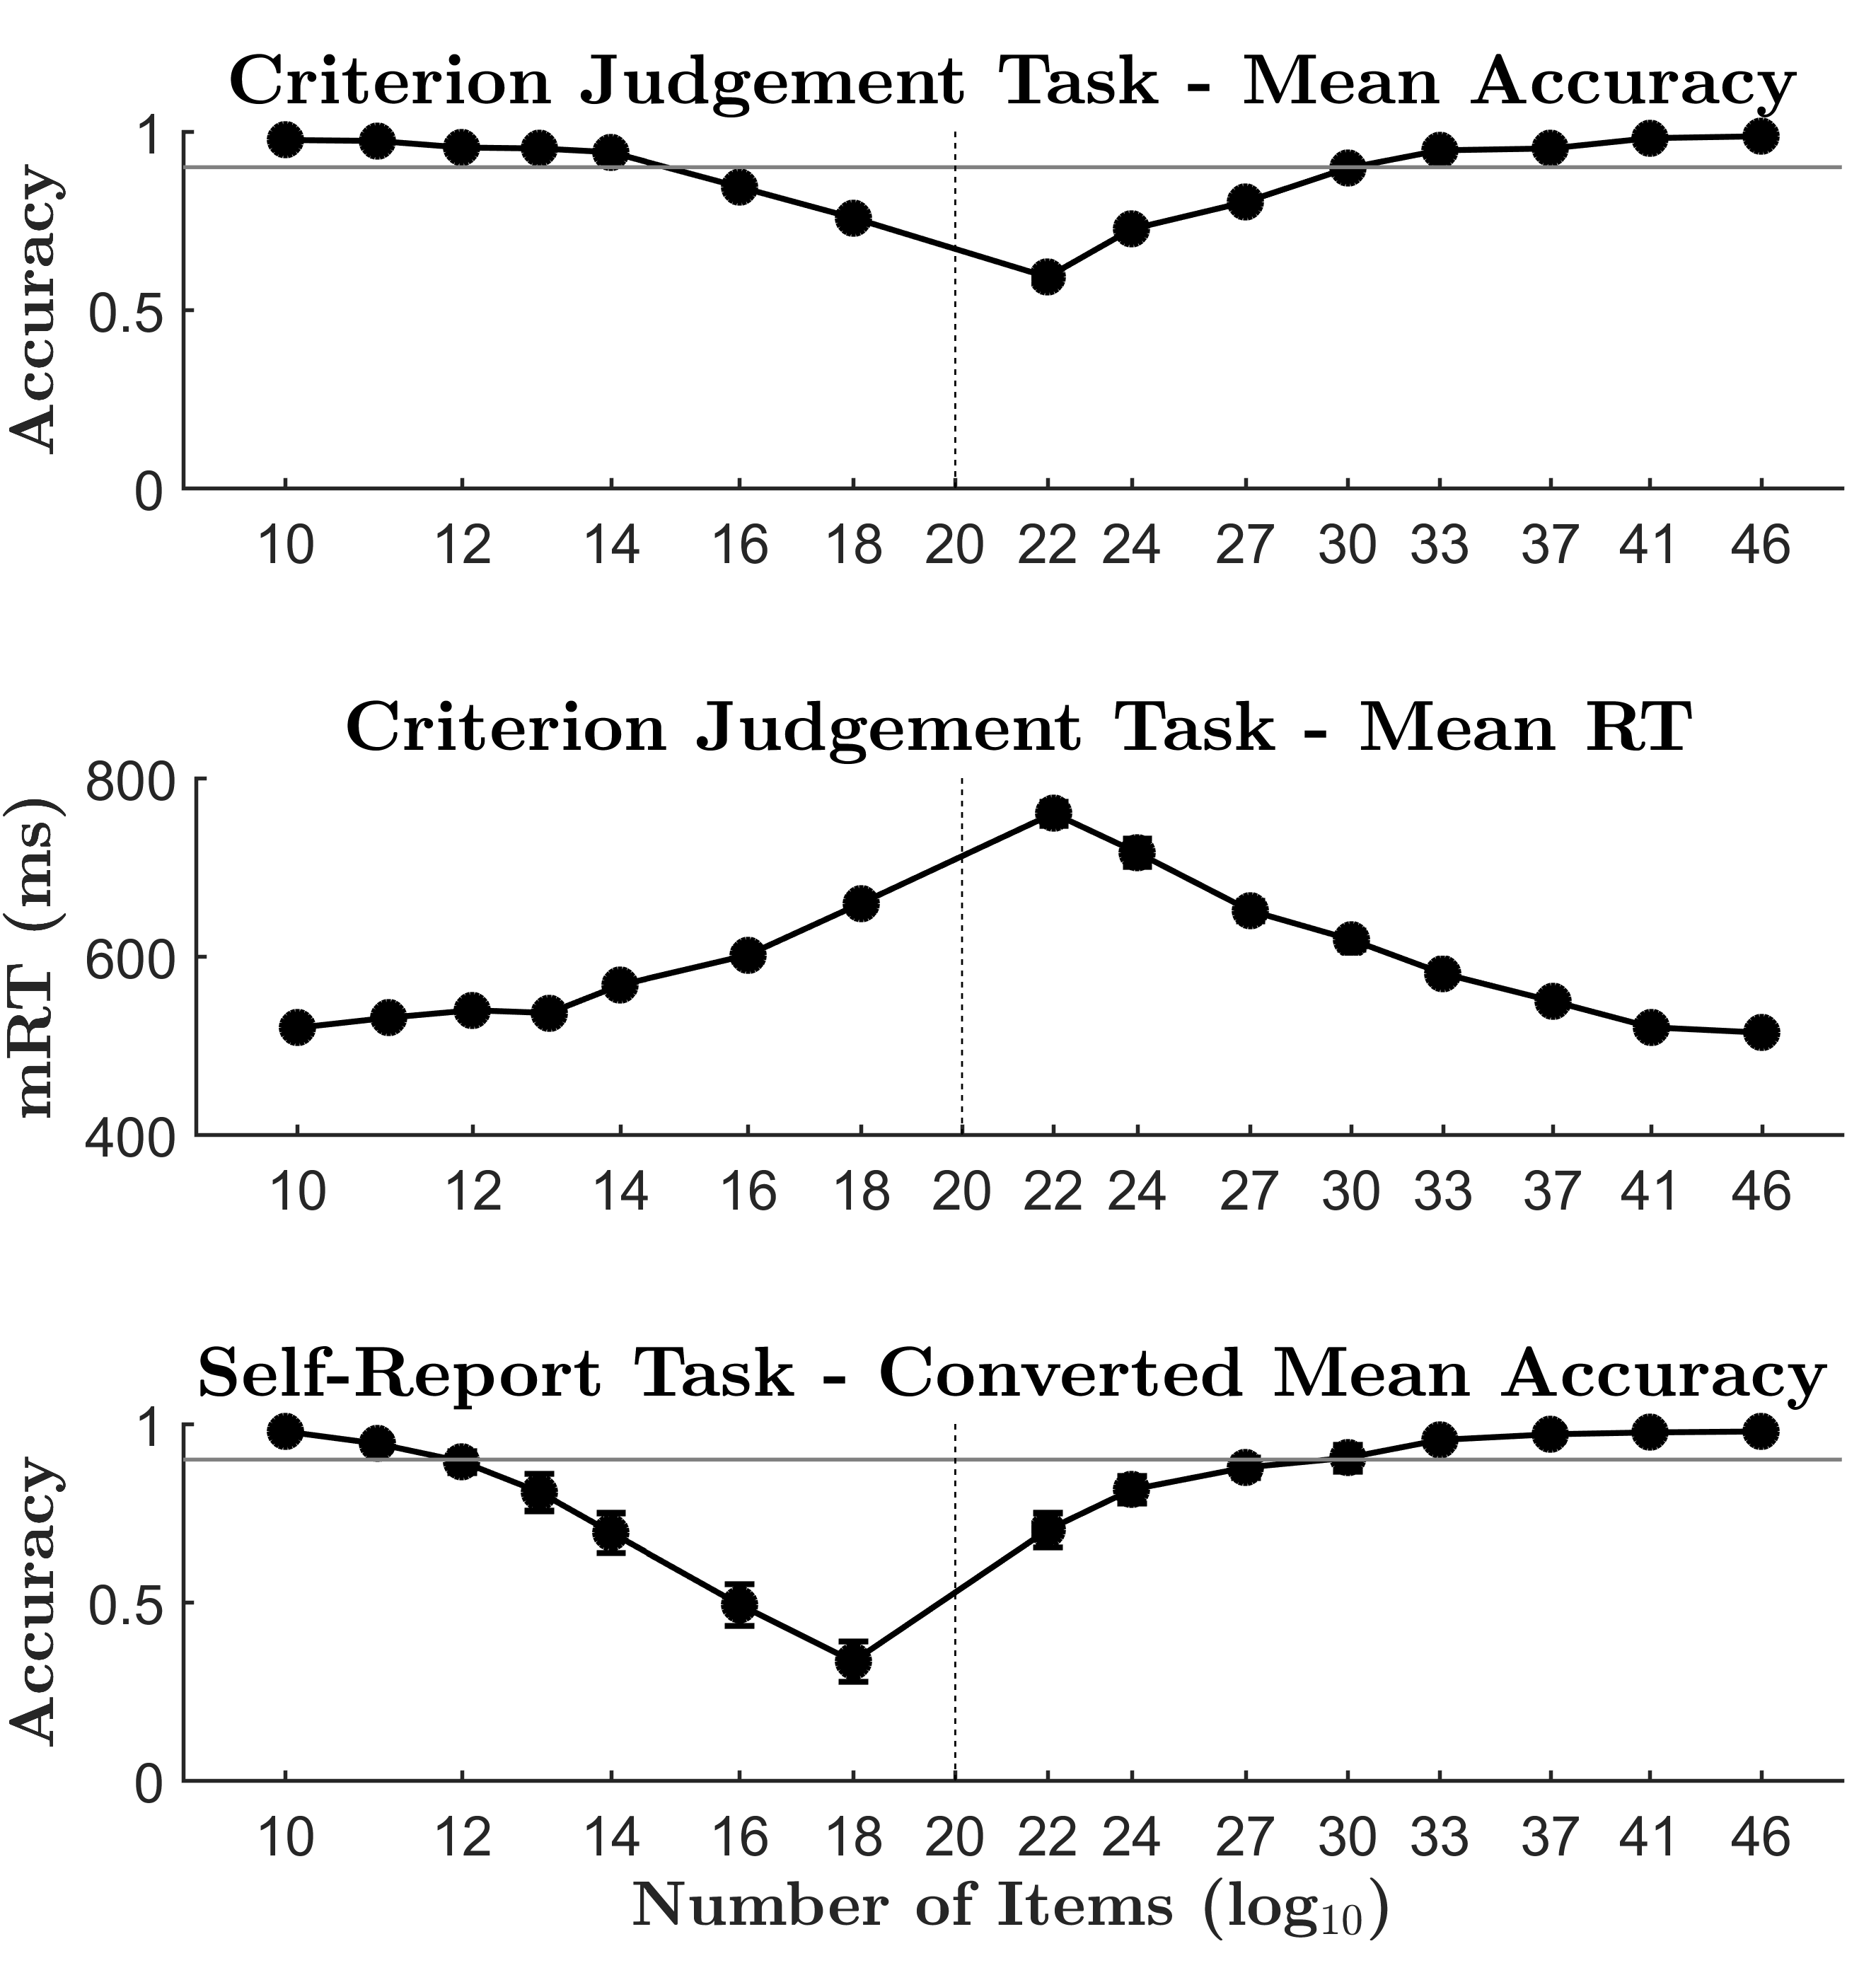
\includegraphics[scale = .75]{Figures/Estimation/FIG15JPG.png}
\caption{Mean accuracy (top) and mean response times (middle) for all participants across set sizes 10-46 in the criterion response-task, and converted mean accuracy (bottom) across set sizes 10-46 for the self-report task. The dotted line represents the response criterion of 20 and the solid horizontal line in accuracy plots illustrates the 90\% threshold. Item set-size is logarithmically spaced along the x-axis. Error bars show $\pm$ one standard error of the mean.}
\label{fig:CritVsExact}
\end{figure}

\subsection{Self-report accuracy vs comparative judgment accuracy}
To compare accuracy between tasks and determine if the ANS was engaged in both tasks, we transformed the self-reported estimates into accuracy scores based on the comparative numerosity task. Correct responses were those that accurately reported the stimulus as either less-than or greater-than 20. These transformed mean accuracy results are displayed in bottom panel of Figure \ref{fig:CritVsExact}. This panel illustrates a trend in accordance with the numerical distance effect. Accuracy is highest at set-sizes 10 ($M$ = 0.98, $SD$ = 0.01) and 46 ($M$ = 0.98, $SD$ = 0.01) and lowest at set-size 18 ($M$ = .33, $SD$ = 0.06). 

On average, accuracy was higher in the criterion judgment task ($M$ = 0.89, $SD$ = 0.12) when compared to the converted-accuracy of the self-report task ($M$ = 0.82, $SD$ = 0.15; $t$(18) = -3.233, $p$ $<$ 0.01). Both tasks illustrate a clear numerical distance effect on accuracy, an effect mirrored by response-time in the criterion judgment task. These trends suggest the numerical distance effect was engaged within both the self-report and criterion-judgment tasks and support the notion that the ANS was engaged in both tasks. 

\subsection{Selection of salience levels}
One purpose of the current experiments was to select high- and low-salience stimulus levels for a double-factorial comparative estimation task. This requires the selection of a high-salience and low-salience target ($<$ 20), and a high-salience and low-salience distractor ($>$ 20). Salience levels were selected based on three criteria. i) Stimulus accuracy must equal or exceed 90\% accuracy, ii) there must be a significant response-time effect between high- and low-salience conditions, and iii) target and distractor salience levels must be separated by the same Weber-fraction. Separating salience levels by the same Weber-fraction should theoretically produce similar numerical distance effects between target salience levels and distractor salience levels.

\subsubsection{Target salience levels}
For target responses ($<$ 20) within the criterion judgment task, accuracy was $\geq$90\% for item-sets 14, 13, 12, 11 and 10 (see the 90\% horizontal line across accuracy plots in Figure \ref{fig:CritVsExact}). Of these item-sets, the 14 item-set is closest to the criteria of 20 and experiences the slowest response-time (see Figure \ref{fig:CritVsExact}). This is in line with the predictions of the numerical distance effect. The 14 item-set differs to the 20 item-set criteria by a Weber fraction of 0.7. Application of this Weber fraction to the 14 item-set returns an equivalent proportional difference of 10 items. Paired samples \textit{t}-test analysis of the group mean response-times revealed a significant difference between set-sizes 14 (\rt{568}{136}) and 10 (\rt{520}{80}; \tval{18}{-4.54}{$<$ .001}). This significant numerical distance effect indicates that the 14 item-set and 10 item-set conditions would be appropriate for the low salience (\ie slow response; 14 item-set) and high salience (\ie fast response; 10 item-set) target conditions within a double-factorial paradigm. 

\subsubsection{Distractor salience levels}
For non-target or distractor responses ($>$ 20), accuracy in the criterion judgment task was $\geq$90\% for item-sets 30, 33, 37, 41 and 46. Given a Weber fraction of 0.7, a low-salience distractor would contain 29 items and a high-salience distractor would contain 41 items. As accuracy was in excess of 90\% for an item-set of 30 items, we accepted 29 items as our low-salience distractor.

Paired samples $t$-test analysis of group mean response-times revealed a significant difference between set-sizes of 30 (\rt{619}{141}) and 41 (\rt{520}{84}; \tval{18}{37.686}{$<$ .01}). This indicates there would be significant response-time difference between our selected levels of low-salience (29 item) and high-salience (41 item) distractors. As these conditions meet our requirements of accuracy and response-time, and adhered to the same Weber-fraction as our target stimuli, we accepted 29 and 41 items as our distractor item-sets for the upcoming double-factorial design.

\color{\Red}
\section{Discussion}
When asked to view a single set of red (alternatively blue) discs, participants were shown to estimate the quantity of items with similar accuracy, by either self-reporting the quantity on a number pad, or by comparing the quantity to a central criterion. The coefficient of variance for self-reported estimates was within the range expected if the ANS was engaged. In the comparative judgment task, a numerical distance effect was observed for both accuracy and mean RT. The distance effect was also observed in the accuracy of the self-reported estimates. Comparable accuracy trends suggest the ANS may have been engaged in both task types. Target and distractor salience levels (item-sets of 10, 14, 29 and 41 discs, to-be compared against a fixed criterion of 20) were selected using data from the criterion judgment task. These levels will be used in the double-factorial design of Chapter 4, when we investigate systems of comparative estimation.

\subsection{ANS engagement}
Estimates made in the self-report task appear to have engaged the ANS. The coefficient of variance fell within the range predicted when the ANS is engaged. This finding is necessary, but not sufficient to prove ANS engagement. In a similar fashion, the numerical distance effect observed in both tasks is necessary, but not sufficient to prove ANS engagement. However, having met these burdens of evidence, and having established similar effects of accuracy in both task types, we speculate that the ANS was engaged in both the self-report and criterion judgement tasks. In Chapter 3, we will expand on this work by developing a double-factorial comparative numerosity task that, based on these experiments, should also engaged the ANS. 

% AE: why is it critical to assume ANS was engaged? as you point out the evidence is weak (necessary but sufficient), so why commit to it?

\subsection{Over vs under-estimation}
Mean accuracy displayed different patterns of over- and under-estimation between tasks. Converted mean accuracy in the self-report task displayed patterns of over-estimation. Conversely, comparative judgments displayed patterns of under-estimation. 

The difference in over and under estimation between task types might reflect a difference in task designs. The comparative judgment task used a singular point of comparison (20 items), where the self-report task allowed free responding and a post-hoc imaginary point of comparison. If the act of comparing items to a criterion resulted in the underestimation of quantity, this effect would be absent in the self-reported data. Determining whether the change from under- to over-estimation is due to the change in task design would require further experimental testing. We leave this as an avenue of future research. 

\subsection{Conclusion}
In this Chapter, participants were asked to freely report their estimates of quantity using a number pad, or compare their estimates of quantity to a pre-determined central criterion. In both tasks, participants appeared to engage their innate approximate number system and displayed clear numerical distance effects for both accuracy and response-time. High and low salience stimuli (item-sets 10, 14, 29 and 41) were selected using these numerical distance effects, and will be applied in the following double-factorial comparative numerosity task. These item sets displayed high accuracy, significant effects of response-time between high and low-levels of salience, and a consistent Weber-fraction of 0.7. The findings of this Chapter are informative for how we estimate a single item-set, however, provide no insight into how we estimate and compare two quantities. In the following Chapter, we will apply these findings to develop a double-factorial comparative numerosity task and apply SFT to address fundamental questions regarding systems of comparative estimation.
\color{black}

% AE: "participants appeared to engage their innate approximate number system "  >>> WHY is it so important to note we engage ANS  


% Paul 2 Ami: I tried to add the 20 item elbow in, but it doesn't actually explain anything about the findings in the data.
%A second account that may explain a shift from over to under estimation may be the interaction between task type and the change in self-reported estimates for items greater than 20. It has long been established that self-reported estimates of quantity are very accurate for items within the range of subitizing ($\leq$ 4) and become increasing less-accurate above this range, producing a response-accuracy `elbow' \cite<see>{kaufman1949subtizing}. In a very recent investigation, \citeA{portley2019second} established a second elbow within the range of estimation for items above and below 20. For quantities above 20, self-reported estimates become increasingly compressed relative to quantities below 20. Although it is likely this finding applied to our self-reported estimates of quantity, it 


% Ami DONE w Chapter 2 -- 29/10/19